\documentclass[titlepage]{article}
\usepackage{graphicx}
\usepackage{amsmath}
\usepackage{mathtools}
\usepackage{float}
\usepackage{subcaption}
\usepackage{caption}
\usepackage{cases}
\usepackage{amssymb}
\usepackage[title]{appendix}
\usepackage{listings}
\setlength{\parskip}{1em}

\author{StatusQuota}
\title{Sunpath Dashboard Application Manual}
\begin{document}
\maketitle
\tableofcontents
\newpage
\section{Introduction}
This manual explains the usage and functionality of the application. For each dashboard component the documentation will include: an overview description and functionality, screenshots of usage, and underlying calculations for values shown, if applicable. Any duplicate calculations or references will be referenced back to the first mention. 

The manual is structured by sections. First, the introduction gives a basic explanation on the overall usage within the application. It is structured as such: access information, application foundation, navigation, data collection, plot features, and table features. Next, the admin and funder bank reconcillation dashboards will be explained with screenshots, descriptions, and how/where the values are being extracted. The scenario modeling dashboard will be explained with screenshots and descriptions for the various admin and vendor details. Finally, an appendix includes any extra details not required for functionality, but it gives more detailed info such as sql queries or python code. 

Also, it is important to note that each time you navigate away from a dashboard the dashboard "'\textbf{resets}" and goes back to original state it was before the user navigated to it. The manual is also located in pdf at location on the server 
\begin{verbatim}
/home/sunpath_tech/Sunpath/manual
\end{verbatim}

\subsection{Access Information}
In order to access the application the user must navigate to the link listed in the following credentials.  The authentication uses Google Oauth technology, and as a result it will ask you to authenticate with a google account email. Once you authenticate, the authentication will be stored into the cookies, and as a result you will no longer be asked to authenticate on the machine until you clear said cookies. The only restriction is that the emails that can be allowed to access the application must be manually inputed into a file on the server. 

The user credentials needed for the test versions for the application are listed below: 
\begin{enumerate}
	\item web application address: http://sunpath.statusquota.co
	\item user email: spfadmn.test@gmail.com
	\item password: webappP@55
\end{enumerate}
This user email also has full permissions for the google oauth client and api dashboard. This shouldn't have to be touched at all. If you want to add emails to the authorized list of emails, the instructions are described below, but all one has to do is add or remove emails from a list. 
\newpage

\subsection{How to Run and Troubleshoot Application}
The process of running the application and dashboard will be automated. However, if something happens and it needs to be restarted manually or edited in anyway I will provide basic instructions in this section. The application was written entirely in Python and hosted on a linode linux server.

\subsubsection{Running Bash Script}
If something goes wrong and the application is not running, go into the root user. First, ensure the named "webapp" screen is listed. You should see the list of screens, similiar to below, available using the following command
\begin{verbatim}
root@localhost:~# screen -ls
There is a screen on:
1063.webapp	(10/16/2018 04:00:00 AM)	(Detached)
1 Socket in /var/run/screen/S-root.
\end{verbatim}
If this is the output proceed with running the bash script
\begin{verbatim}
root@localhost:~# bash application_script.sh
\end{verbatim}
This will quit the current window and create a new window with the name "webapp" and will run the application. The name for the screen must be "webapp" in order for the automation to work correctly.

However, if the screen does not exist and you get 
\begin{verbatim}
root@localhost:~# screen -ls
No Sockets found in /var/run/screen/S-root.
\end{verbatim}
Then create a detached screen called webapp and then run the bash script using the following commands to restart the server. If there are any other issues, the following section goes into step-by-step directions on how to access the application and run it manually. 
\begin{verbatim}
root@localhost:~# screen -dmS webapp 
root@localhost:~# screen -ls
There is a screen on:
4481.webapp	(10/16/2018 06:01:15 PM)	(Detached)
1 Socket in /var/run/screen/S-root.
root@localhost:~# bash application_script.sh 
\end{verbatim}

\subsubsection{Basics and Troubleshooting}
In order to access the server, one should follow online instructions for ssh. Once you have access if you are on the root user  you can either resume a screen. This command lists available screens and should display the following
\begin{verbatim}
root@localhost:~# screen -ls
There is a screen on:
550.webapp	(09/12/2018 10:04:17 PM)	(Detached)
1 Socket in /var/run/screen/S-root.
\end{verbatim}
If no screens are listed, then you can start a screen with a name (this example will use the name "test"). You start a new screen proceed to the instructions for navigating to the webapp user in order to access application or start it.
\begin{verbatim}
root@localhost:~# screen -S test
\end{verbatim}
If you ever have to kill a specific screen, use the command. 
\begin{verbatim}
root@localhost:~# screen -X -S test quit
\end{verbatim}
However, if you want to resume a screen 
\begin{verbatim}
root@localhost:~# screen -r test
\end{verbatim}
In order to detach from a screen so it can run in the background just hit "Ctrl + a then d". If you have any issues, I would suggest looking up more instructions online. 

Once you are on the sunpath\_tech user, you should then navigate to the home directory. 
\begin{verbatim}
sunpath_tech@localhost:/root$ cd
\end{verbatim}
Once in the home directory, you should activate the virtual environment. Below showcases how to do this via command terminal, and the virtual environment should be activated. To ensure this, it will display "(webapp\_env)" to ensure the virtual environment is activated. 
\begin{verbatim}
sunpath_tech@localhost:~$ source webapp_env/bin/activate
(webapp_env) sunpath_tech@localhost:~$ 
\end{verbatim}
In order to activate the application and dashboard, run the following command into the console.
\begin{verbatim}
gunicorn -b 0.0.0.0:8050 --timeout 240 --chdir /home/sunpath_tech/Sunpath index:app.server
\end{verbatim}
if successful, you should see 
\begin{verbatim}
[2018-10-12 15:49:32 +0000] [28455] [INFO] Starting gunicorn 19.9.0
[2018-10-12 15:49:32 +0000] [28455] [INFO] Listening at: http://0.0.0.0:8050 (28455)
[2018-10-12 15:49:32 +0000] [28455] [INFO] Using worker: sync
[2018-10-12 15:49:32 +0000] [28459] [INFO] Booting worker with pid: 28459
\end{verbatim}

\subsubsection{Adding Emails to Authorized Emails List}
The authorized email list is located at the path and file
\begin{verbatim}
/home/sunpath_tech/Sunpath/static/authorized_emails.py
\end{verbatim}
To add or remove emails, you just have to include the email listed in the list. The authorization uses Google Authorization. In case anything happens with Google and this needs to be accessed, you can access this in the Google API console using the user listed in the manual. But it can be accessed with this link 
\begin{verbatim}
https://console.cloud.google.com/apis/
credentials?authuser=5&folder&organizationId&project=sunpath-206919
\end{verbatim}

\subsubsection{Other Important Information}
Most of the instructions listed in the previous section can get you to restarting or navigating to the application location. Also, you can terminate the application from root user via command 
\begin{verbatim}
pkill gunicorn
\end{verbatim}
or navigating to the screen with the application running and terminating it manually "Ctrl + C". 

If the data stops updating for whatever reason, something may have changed database-side. If that is the case the scripts that are used to update the data are located in the following path.
\begin{verbatim}
/home/sunpath_tech/Sunpath/static/scripts
\end{verbatim}
The data is saved to location at 
\begin{verbatim}
/home/sunpath_tech/Sunpath/static/data
\end{verbatim}

If the automation doesn't seem correct or needs adjusting, you can adjust the crontabs in the sunpath\_tech and root user account. The times for updating the data are between 12-4am. You can access the crontabs via the command
\begin{verbatim}
crontab -e
\end{verbatim}
The webapp user's crontab is shown below. It runs the scripts to update controls like sellers, funders, and any other variables and definitions, expected values for forecasting, scenario modeling tables and data, and bank reconcillation tables and data. /textbf(The bank reconcillation script is currently commented out because the SPAdmin database is not located in the database location. So once it is available, all someone has to do is go in and uncomment it out to run.) 
\begin{verbatim}
0 0 * * *       /home/sunpath_tech/webapp_env/bin/python 
/home/sunpath_tech/Sunpath/static/scripts/update_controls.py
2 0 * * *       /home/sunpath_tech/webapp_env/bin/python 
/home/sunpath_tech/Sunpath/static/scripts/generate_expected_values.py
0 3 * * *       /home/sunpath_tech/webapp_env/bin/python 
/home/sunpath_tech/Sunpath/static/scripts/generate_scenario_modeling_data.py
#30 3 * * *     /home/sunpath_tech/webapp_env/bin/python 
/home/sunpath_tech/Sunpath/static/scripts/generate_bank_recon_data.py
\end{verbatim}
The root user crontab runs the script that was mentioned in a previous section. It resets the application at 4am in order to use the new updated data.
\begin{verbatim}
0 4 * * * bash application_script.sh
\end{verbatim}

\subsection{Plotly/Dash}
The application foundation uses the python framework known as Dash. Dash uses the Plotly framework for visualizations. It is a web-based interface that is used for building interactive analytical web applications. It uses various UI elements like dropdowns, sliders, and graphs in combination with Python code. This allows for a very powerful tool that can combine web-based applications with coding elements. As a result, it provides a foundation for interactive visualizations in a medium that can be simple, easy to use and learn.  

\subsection{Navigation}
The "Home Page" will be the main portal/location to navigate the various dashboard components. Each dashboard component has a link in the top left corner that will directly take the user back to the home page. When a user wants to navigate to a dashboard, they must click on the link to the desired dashboard component at the home page. \textbf{It is important that one must select the "Home Page" link to navigate back to the home portal in order to load the page. This is to insure correct loading of application elements.}

\subsection{Data Collection and Information}
The data for the application is gathered directly from csv files that are generated by scripts. The scripts generate csv files from querying commands from the Sunpath database \textbf{SPAdmin} and \textbf{FundingPaylink\_Live}. As long as the Sunpath database is updated, so will the data that is shown in the dashboards. Here is a list of databases, tables, and the corresponding dashboards assocaited with the table:

Database: \underline{\textbf{SPAdmin}}
\begin{enumerate}
	\item SPA\_SPBankingStat (Bank Reconcillation)
	\item SPA\_SPDepositsStat (Bank Reconcillation)
	\item SPA\_Funded\_Contracts (Bank Reconcillation)
	\item SPA\_SPPlugStat (Bank Reconcillation)
	\item SPA\_SPPaymentsStat (Bank Reconcillation)
\end{enumerate}

Database: \underline{\textbf{FundingPaylink\_Live}}
	\begin{enumerate}
		\item SPF\_Funding\_Transaction\_Log (Bank Reconcillation, Scenario Modeling)
		\item SPF\_Funding\_Transaction\_Codes (Bank Reconcillation, Scenario Modeling)
		\item Daily\_Extract(Scenario Modeling)
		\item Admin\_Funding (Scenario Modeling)
		\item Seller\_Funding (Scneario Modeling)
		\item StoneEagle\_All\_Customer\_Info (Scenario Modeling)
		\item Seller\_Info\_Funding\_Approved\_Partners (Scenario Modeling)
		\item Seller\_Info\_Funding\_Parameters (Scenario Modeling)
	\end{enumerate}
	
\subsection{Plot/Graph Visuals and Features}
The visualizations and plots generated from the application and dashboards can be interacted with by the user. All plots and visuals have the following attributes: hover tool, functionality features (zoom, pan, box select, axes reset and autoscale), download to png, ability to edit in plotly's chart studio, and much more. A convenient toolbar is visible once the user hovers on the visual. 

\subsection{Table Visuals and Features}
Most tables in the application also come with some basic customizable features. A user can take a column header and resize to their preferred width. Also, a user can sort a table by selecting a column header and choose to sort by ascending or descending values. And unless specificed, some tables allow the user to edit the table by choosing their own input values. 
%---------------------------------------------------------------------------
\newpage
\section{Admin Bank Reconcillation}
\subsection{Summary}
This dashboard component allows the user to see the admin version of the bank reconcillation summary dashboard. It shows a table and column names for "Bank of America" and "Sunpath" tables. The "Bank of America" columns are the various descriptions for account types: $Days/Months$, $Ops$, $Claims$, $INS$, $Payroll$, $Escrow$, and $Total$. The "Sunpath" columns are the types/database tables : $Days/Months$, $Deposits$, $Insurance$, $Plugs$, $Packs$ $Payments$, and $Total$. The $Variance$ column value is the difference between the "Bank of America:$Total$" and "Sunpath:$Total$".

\subsubsection{How to Use}
\begin{enumerate}
	\item Edit the Date Range for the "Clear Date" by selecting the dates in the dropdown calendar. One can also modify the view to show "Days" or "Months"
	\begin{figure}[h]
		\begin{subfigure}[b]{.5\textwidth}
			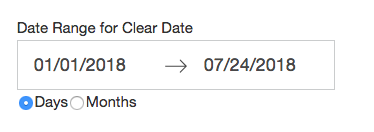
\includegraphics[scale=.5]{./pics/bank_reconcillation_dateRange.png}
		\end{subfigure}
		~
		\begin{subfigure}[b]{0.5\textwidth}
			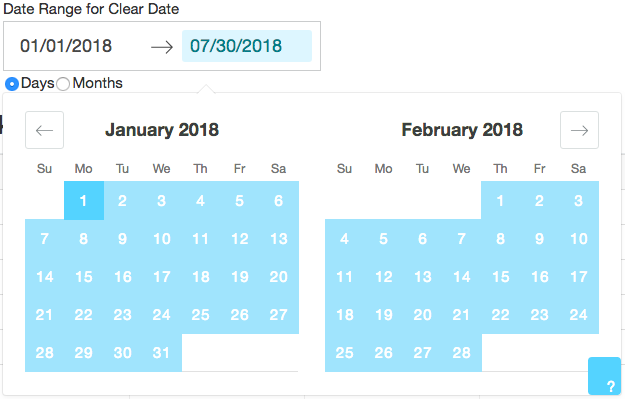
\includegraphics[scale=.3]{./pics/bank_reconcillation_dateRange_dropdown.png}
		\end{subfigure}
	\end{figure}
	\item Once a date range is selected, the table will fill with necessary information, which can be scrollable
\end{enumerate} 
\subsubsection{Value Definitions}
For the Bank of America table, the column values: $Ops$, $Claims$, $INS$, $Payroll$, and $Escrow$ are $Account$ types within the \textbf{SPA\_SPDepositsStat} database table. The Bank of America's rows are organized by days or months starting from the first $Clear Date$ in the selected date range. The Bank of America account's values are the sums from the $Amount$ column in the database table on the selected day or month. The Bank of America column $Total$ is defined as 
\begin{equation} \label{eq:1}
Total = Ops + Claims + INS + Payroll + Escrow
\end{equation}
Similarily, the Sunpath table is organized by day or month. The Sunpath column values: $Deposits$, $Insurance$, $Plugs$, and $PacksPayments$ are taken from the database tables \textbf{SPA\_SPDepositsStat}, \textbf{SPA\_Funded\_Contracts}, \textbf{SPA\_SPPlugStat}, and \textbf{SPA\_SPPaymentsStat}. The values are sums of either the $PaymentAmount$ or $Amount$ columns in the database tables except for $Insurance$, where the value is taken from $InsuranceReserveAmount$ in the database table. The Sunpath total is defined as 
\begin{equation}\label{eq:2}
Total = Deposits + Insurance + Plugs + Packs Payments
\end{equation}
The final value $Variance$ is defined as the difference between these two totals
\begin{equation}
Variance = \text{equation \ref{eq:1}} - \text{equation  \ref{eq:2}}
\end{equation}

\subsection{Details}\label{adminbankdetail}
This dashboard component shows the detail summary of the various tables/account types/tables: Plugs, Deposits, Payments, Insurance, Banking Transaction. The details help provide basic summaries and include further notes, descriptions, payee, vendor, and/or group name associated with the specific amount in the database entry. In order to provide this more detail summary, the date range can only be organized by $ClearDate$ in units of days. Due to the size of the tables, all tables are displayed and can be scrolled through. 
\subsubsection{How to Use}
\begin{enumerate}
	\item Edit the Date Range for the "Clear Date" from the dropdown calendar.
	\begin{figure}[h]
		\begin{subfigure}[b]{.5\textwidth}
			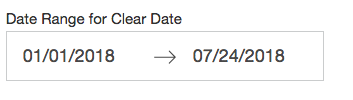
\includegraphics[scale=.5]{./pics/bank_reconcillation_dateRange_detail.png}
		\end{subfigure}
		~
		\begin{subfigure}[b]{.5\textwidth}
			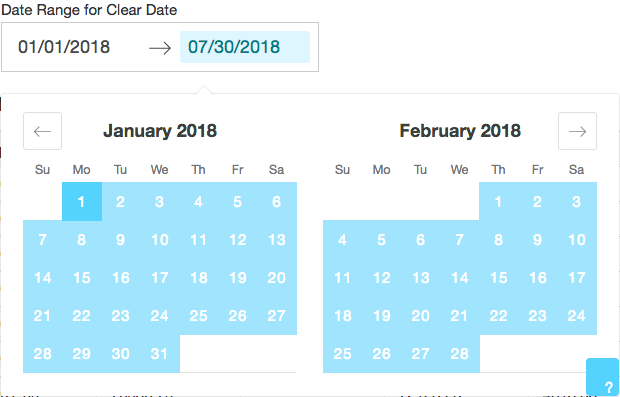
\includegraphics[scale=.3]{./pics/bank_reconcillation_dateRange_dropdown_detail.png}
		\end{subfigure}
	\end{figure}
	\item Information will be filled in the tables once a date range is selected.
\end{enumerate}
\subsubsection{Value Definitions}
All tables and values were generated using the sql queries found in appendix \ref{appendix:sql1} at the end of the document. Some values were renamed, such as disbursetype to groupname, PaidTo to Payee, etc. This can all be seen in the appendix. 
%---------------------------------------------------------------------------

\section{Funder Bank Reconcillation}
\subsection{Summary}
This dashboard component shows info intended for the funder side of the business. It functions and operates similiarily to the admin component, but differs in the information shown. It shows the user the totals for the various types/accounts for each day or month and shows the variance between the totals from the accounts and the bank amount total from the transaction logs. The transaction logs were organized using the sql query in appendix \ref{appendix:sql2}. The data collected is from the database tables \textbf{SPF\_Funding\_Transaction\_Log} and \textbf{SPA\_FundingBankStat}.

\subsubsection{How to Use}
\begin{enumerate}
	\item Edit the Date Range for the "Clear Date" from the dropdown calendar. One can also modify the view to show "Days" or "Months"
	\begin{figure}[h]
		\begin{subfigure}[b]{.5\textwidth}
			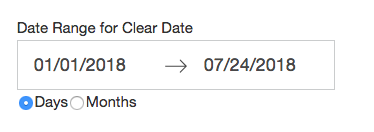
\includegraphics[scale=.5]{./pics/bank_reconcillation_dateRange.png}
		\end{subfigure}
		~
		\begin{subfigure}[b]{0.5\textwidth}
			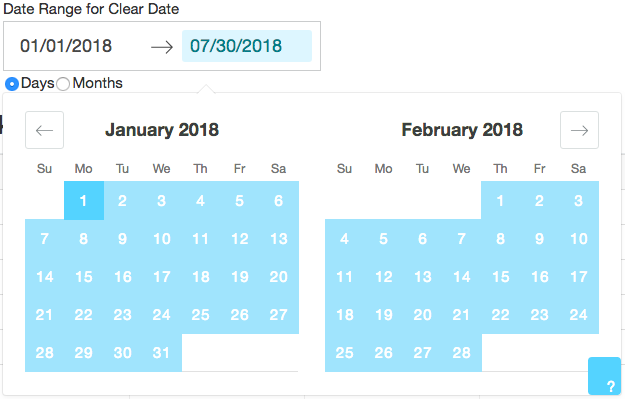
\includegraphics[scale=.3]{./pics/bank_reconcillation_dateRange_dropdown.png}
		\end{subfigure}
	\end{figure}
	\item Once a date range is selected, the table will fill with necessary information, which can be scrollable
\end{enumerate} 

\newpage
\subsection{Value Definition}
As mentioned, the data collected is from the database tables \textbf{SPF\_Funding\_Transaction\_Log} and \textbf{SPA\_FundingBankStat}. The $BankAmtTotal$ is collected from the \textbf{SPA\_FundingBankStat}. The second table's values are compiled through the transaction log's $TxDescription$ and $TxAmount$. The $Total$ for each day is the addition of all the values, defined as:
\begin{equation}
\begin{split}
Total &= DepositsAmt + InsuranceAmt + PaymentAmt \\
&+ PlugAmt + CustCollAmt + CollectAmt
\end{split}
\end{equation}The $Variance$ is the difference between the $BankAmtTotal$ and $Total$:
\begin{equation}
Variance = BankAmtTotal - Total
\end{equation}

\subsection{Details}
Similar but slightly different to the admin bank reconcillation section details \ref{adminbankdetail}, it includes accounts/types from customer collections and collections and the details were gathered from different tables. The tables shows the $Amount$ grouped by the $ClearDate$, $Description$, and/or $Vendor$

\subsubsection{How to Use}
\begin{enumerate}
	\item Edit the Date Range for the "Clear Date"
	\begin{figure}[h]
		\begin{subfigure}[b]{.5\textwidth}
			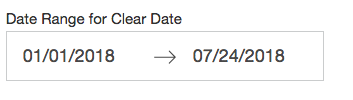
\includegraphics[scale=.5]{./pics/bank_reconcillation_dateRange_detail.png}
		\end{subfigure}
		~
		\begin{subfigure}[b]{.5\textwidth}
			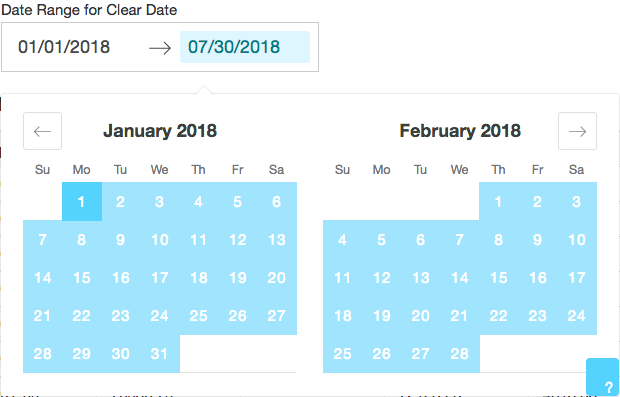
\includegraphics[scale=.3]{./pics/bank_reconcillation_dateRange_dropdown_detail.png}
		\end{subfigure}
	\end{figure}
	\item Information will be filled in the tables once a date range is selected.
\end{enumerate}
\newpage
\subsubsection{Value Definitions}
In order to seperate the descriptions into their respective account types within the database table \textbf{SPA\_FundingBankStat}. A key was created to assist in this process. Currently, this key is static. Any new descriptions would require manual updating/editing. The description key is defined as 
\begin{verbatim}
DESCR_KEYS = 
Administrator Funding : Deposits,
Insurance Reserve Funding : Insurance,
Paylink Chargeback Fee : Customer Collections,
Paylink Customer Collection : Customer Collections,
Paylink Customer Collection Reversal : Customer Collections,
Paylink Processing Fee : Customer Collections,
Paylink Processing Fee Reversal : Customer Collections,
Paylink Returned Payment Fee : Customer Collections,
RC (Debit Seller Wire) : Deposits,
Returned Premium - Admin : Deposits,
Returned Premium - Ins Reserve : Deposits,
Reverse Administrator Funding : Payments,
Reverse Insurance Reserve Funding : Collections,
Reverse Returned Premium - Admin : Collections,
Reverse Returned Premium - Ins Reserve : Collections,
Reverse Seller Funding : Collections,
Seller Funding : Payments
\end{verbatim}

%---------------------------------------------------------------------------
\newpage
\section{Scenario Modeling}
The scenario modeling dashboards consist of three components: summary, admin details, and vendor details. 
\subsection{Summary}
This dashboard component consists of values and visuals to give the user a basic summary of a vendor, funder cohorts. The values shown are "Total Contracts Sold", "Total Face Value Sold", "Avg. Contracts Sold, Month", "Avg. Face Value", "Total Seller Advance Received", "Avg. Contracts Sold, 3 Months", and "Growth Rate, M-O-M (Recent ,Complete)." The two interactive visuals show the Cohort's Month Sales Volume and the Cohort's Current Cancel Rates per Payments Made. 
\subsubsection{How to Use}
\begin{enumerate}
	\item Click on the arrow to toggle the funder field from visible and not visible. In the field, the user can select 1 or more funders from the dropdown list
	\begin{figure}[h]
		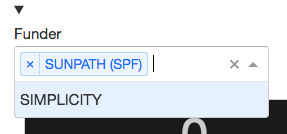
\includegraphics[scale=.5]{./pics/scenario_modeling_funder.png}
	\end{figure}
	\item Click on the second arrow and toggle the vendor field from visible and not visible. In the field, the user can select 1 or more funders from the dropdown list
	\begin{figure}[h]
		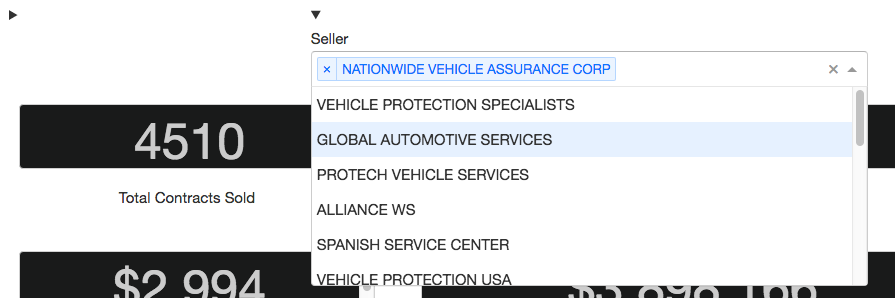
\includegraphics[width=\linewidth]{./pics/scenario_modeling_seller.png}
	\end{figure}
	\item The fields will fill with numbers and the visuals will display 
\end{enumerate}
\subsubsection{Visuals and Plots}
\begin{enumerate}
	\item The cohort's monthly sales volume shows the count vs. month and year. The plot separates counts by cancelled, open, and completed contracts
	\begin{figure}[h]
		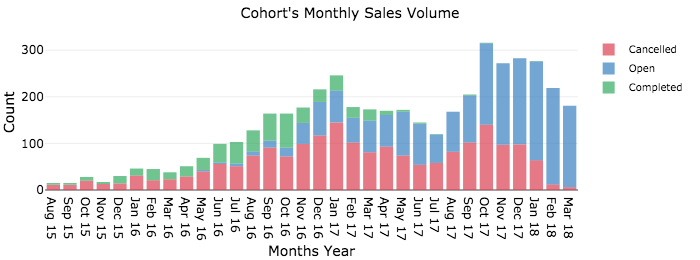
\includegraphics[scale=.5]{./pics/monthly_sales_vol.png}
	\end{figure}
	\item the cancel rates per payments made shows the selected vendor cancel rates compared with all the vendors. Also the user can select 1 or more cohort(installment term lengths) to look at specific contract terms and displayed above each bar/bin is the percent(rounded).
	\begin{figure}[h]
		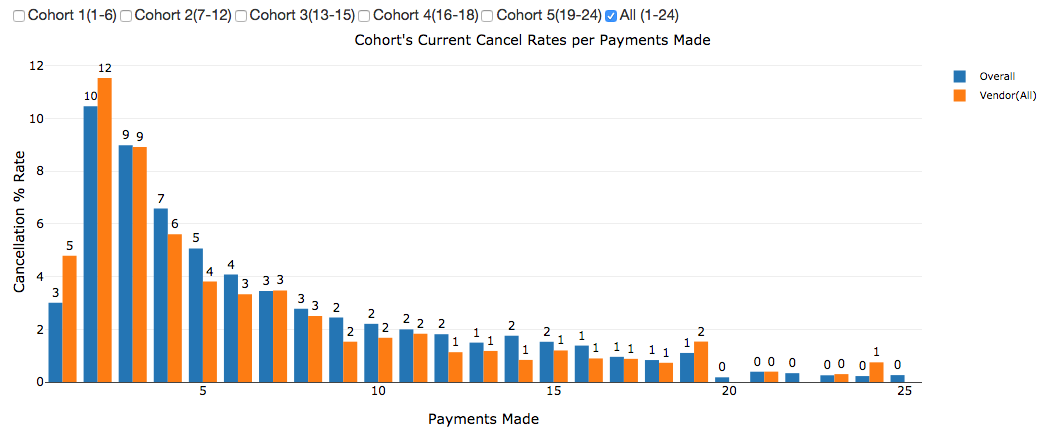
\includegraphics[scale=.4]{./pics/cancellation_rate_paymentMade.png}
	\end{figure}
\end{enumerate}

\newpage
\subsubsection{Value Definitions and Calculations}
The cancel curve plot visual is created by using rules from the cancelillustration.pdf; a brief example is shown below.
\begin{figure}[h]
	\centering
	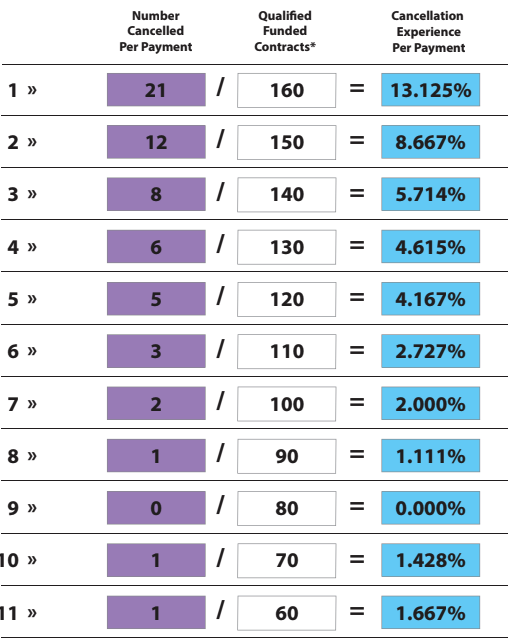
\includegraphics[scale=.3]{./pics/cancel_curve_ex.png}
\end{figure}
The numerator is defined as "Number Cancelled Per Payment" and the denominator is defined as "Qualified Funded Contracts", which is defined below in a small figure. 
\begin{figure}[h]
	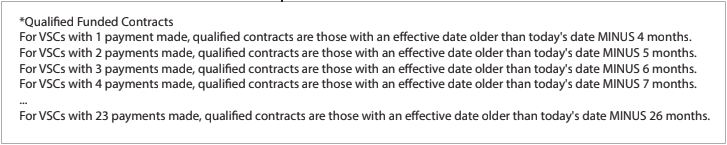
\includegraphics[scale=.4]{./pics/cancel_curve_qfc.png}
\end{figure}
The resulting fraction is the "Cancellation Experience Per Payment."

The monthly sales volume histogram's bins for a cohort are calculated by grouping by month, year and contract status: completed, cancelled, or open. Finally, the values shown in fields are calculated and defined as:
\begin{enumerate}
	\item Total Contracts Sold = Total \# contracts in a cohort's historical data
	\item Total Face Value Sold = Total amount financed from all contracts in a cohort's historical data
	\item Avg. Contracts, Month = The mean or average number of contracts sold per month based on a cohort's historical data
	\item Avg. Face Value = The mean or average amount financed for a contract based on a cohort's historical data
	\item Total Seller Advance = Total Seller Advance Amount from each contract based on a cohort's historical data
	\item Avg. Contracts Sold, 3 last months = The mean or average number of contracts sold in the most recent 3 months of a cohort
	\item Growth Rate = Calculates the rate of contracts sold from 2 months from the most recent month. Example. if now = April 2018, we look at the growth rate from January 2018 to Feburary 2018. This was chosen because 2 months from the most recent month allowed the database to be properly updated with data.  
\end{enumerate}

\subsection{Admin and Vendor Details}\label{admin}
This dashboard component contains the tables and values for admin or vendor details. The admin dashboard component includes "Loss Ratio" and "Expected IRR" columns in the tables, but the vendor component does not include these. Also, a general rule is applied for sellers that do not have many contracts under their historical performance. If a seller or cohort has less than 75 contracts then we use a "Sunpath Average", which uses the data from taking all the contracts in Sunpath's historical database. 

\textbf{\emph{Note 1:} Some of the fields will not load on first time data is calculated, depending on the data queried. This can easily be solved by reselecting the seller, funder, or editing an editable field and hitting "Enter" to reload and recalculate.}

\textbf{\emph{Note 2:} For the purpose of this manual and section, a funder and seller combination will be defined as a group and the installment terms will be defined as a cohort.}
\subsubsection{How to Use}
\begin{enumerate}
	\item Click on the arrow to toggle the funder field from visible and not visible. In the field, the user can select 1 or more funders from the dropdown list
	\item Click on the second arrow and toggle the vendor field from visible and not visible. In the field, the user can select 1 or more funders from the dropdown list
	\item The user can modify the "Contract Fee" value by changing the field (Default is 50)
	\begin{figure}[h]
		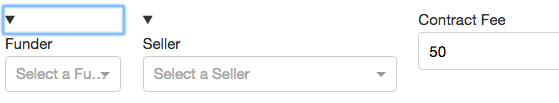
\includegraphics[width=\linewidth]{./pics/scenario_modeling_toggle.png}
	\end{figure}
	\item The fields will fill with numbers and the visuals will display, this may take a few seconds where the length it takes to load depends on the cohort's data 
	\item The leftmost columns: "Cancel Reserve \%", "Discount Amount \%", and "Contracts,Month" can be modified \textbf{Highlighted in Red}
	\item Changing these values will modify the columns corresponding to the related related table on the right \textbf{Highlighted in Blue}
	\begin{figure}[h]
		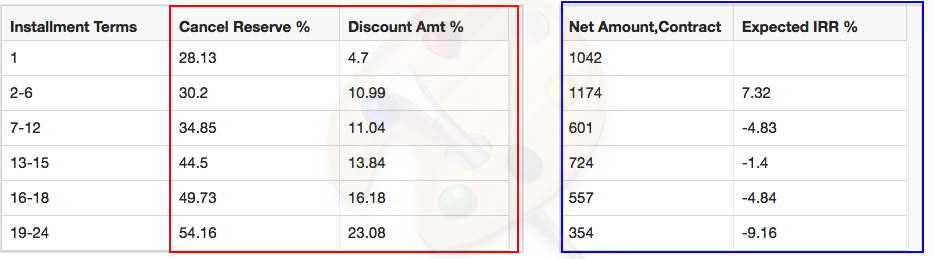
\includegraphics[width=\linewidth]{./pics/scenario_modeling_admin_firstTable.png}
	\end{figure}
	\begin{figure}[h]
		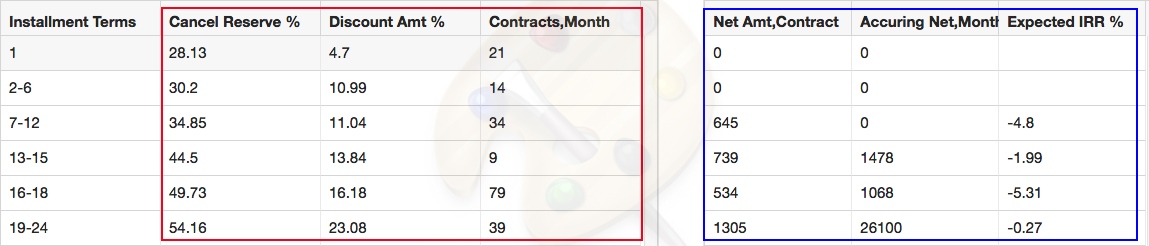
\includegraphics[width=\linewidth]{./pics/scenario_modeling_admin_secTable.png}
	\end{figure}
\end{enumerate}
\newpage
\subsubsection{Values Definitions and Calculations}
This section gives the description and calculations for this dashboard's values. Basic summary of the values are defined below, where a cohort is defined as the installment term range:
\begin{enumerate}
	\item Installment Term: Funder \& Vendor groups divided by contract term lengths 1,2-6,7-12,13-15,16-18,19-24
	\item Contract Sold: Number of contracts sold in the installment term cohort
	\item \% Contracts Sold:  Percent of contracts sold
	\item Cancel Reserve \%: Cancel reserve amount percent
	\item Discount Amount \%: Discount amount percent
	\item Net Amount: The net surplus or deficitfor the installment term cohort
	\item Loss Ratio: $\frac{APR + EPR}{\text{Total Cancel Reserve Amount}}$
	\item Net Amount, Contract: The net surplus or deficit per contract in installment term cohort
	\item Current IRR \%: The internal rate of return as a percentage for contracts in the cohort up to their current state (this is not a projection)
	\item Cumulative Net Deficit/Surplus: The Cumulative Net Surplus or Deficit amount for the funder, seller group
	\item Cumulative Cancel Reserve: The total cancel reserve for the funder, seller group
	\item Avg. Contracts Sold, Month: The average contracts sold per month for the funder, seller group
	\item Contracts, Month: This editable field is the number of contracts sold per month to calculate the accuring net holdback per month
	\item Net Amt, Contract: The net deficit or surplus amount on a per contract basis for the installment term cohort
	\item Accruing Net, Month: The accruing net holdback per month based on the net holdback amount per contract
\end{enumerate}
The calculations for many of these values will be shown below, as well as the variables used in the calculations:
\begin{enumerate}
	\item $TermDays$ = term of a contract in days
	\item $EffectiveDate$ = the Effective Date of a contract
	\item $DueDate$ = the due date of next payment for a contract
	\item $CancelRsv$ = cancel reserve of a contract
	\item $SellerCost$ = the seller cost of a contract
	\item $SellerAdvance$ = seller advance for a contract
	\item $InstallAmt$ = installment amount for a contract
	\item $DiscountAmt$ = discount amount of a contract
	\item $PaymentsMade$ = the total payments paid by customer for a contract
	\item $TotalCancelRsvAmt$ = the total cancel reserve amount for cohort
	\item $ProbNC$ = probability of a contract not cancelling
	\item $ProbC$ = probability of cancelling
	\item $RP$ = returned premium (unweighted)
	\item $Term$ = a contract installment term length
	%\item $fee$ = contract fee (this is found on Page 14 of the Sunpath Workflow Document provided to us)
	\item $AdminFundAmt$ = admin funding amount
	\item $InsRsvAmt$ = insurance reserve funding amount
	\item $APR$ = $InstallAmt \times PaymentsMade$ for cohort
	\item $EPR$ = total expected projected receivable for cohort
	%\item $DayUtilized$ = Cancel Date - Effective Date of a contract in days
	%\item $VUR$ = $\frac{DayUtilized}{TermDays}$
	\item $VendorRate$ = vendor specific rate
	\item $ProratedFee$ = $VendorRate \times DiscountAmt$
	\item $AmountFinanced$ = amount financed for a contract
	\item $InstallAmtRec$ = $InstallAmt \times PaymentsMade$, amount received currently for a contract
	%\item $AmtOwedSPF$ = $(1-VUR)(AdminFundAmt) - fee$
	%\item $AmtOwedIns$ = $(1-VUR)(InsRsvAmt)$
\end{enumerate}
The main calculation for $NetSurplusDeficit$ is different, depending on if a contract cancels or completes:
\begin{equation}
\begin{split}
NetSurplusDeficit = Total + ReturnedPremium
\end{split}
\end{equation}
where $Total$ and $ReturnedPremium$ is defined as
\begin{equation}
	\begin{split}
	SellerAdvance &= AmountFinanced - (SellerCost + DiscountAmt + CancelRsv)\\
	Total &= -(AdminFundAmt + InsRsvAmt\\
	&+ SellerAdvance + ProratedFee - InstallAmtRec)
	\end{split}
\end{equation}
\begin{equation}
\begin{split}\label{returnedprem}
Fraction(Days) &= \left[\frac{TermDays + \left[EffectiveDate - (DueDate + 30 days)\right]}{TermDays}\right]\\
ReturnedPremium &= Fraction(Days) \times SellerCost - 50
\end{split}
\end{equation}
The $ExpectedValue$ is the expected projected receivable for an contract at some payment $i$ in its lifetime. A cancelled contract's expected value would be the returned premium that is taken from contract fields within the database. A completed contract would not expect any further payment. Finally, an open contract would expect to receive payments up to the last payment, $j$, and if it cancels it would have a returned premium, which is calculated from equation \ref{returnedprem}. 

The expected projected receivable is a function of a contract's $InstallAmt$, $Term$, $PaymentsMade$, $EffectiveDate$, and $SellerCost$ for returned premium calculation. The method and algorithm utilizes a Monte Carlo to create a simulation of contracts with installment term $N = 1,2,3,4,...,24$. It uses the contracts within the database to calculate the conditional probabilities for contracts with term $N$ given installments paid $i$. It uses these probabilities to run a simulation for each individual contract term 100,000 times, and then uses the information to get an expected last payment $j$ as a function of term $N$ and installments paid $i$. The value used for last payment is one standard deviation above the mean, as this value gave us the "best" precision based on backtesting analysis between 50\%-80\% depending on the contract term , a contract's lifetime, and the amount of contracts in the backtesting cohort. 
\begin{equation}
last\ payment= Probability(N,i)
\end{equation}
%\begin{equation}
%\begin{split}
%ExpectedValue &= InstallAmt \times ProbNC \\
%&+ RP\left(\frac{Term-i}{Term}\right) \times ProbC
%\end{split}
%\end{equation}

The IRR calculation uses a built in function available in Python. This is not a projection as that would be beyond the dashboard's purpose, and a projected IRR would require more time and computation power that is not available with a real time calculation product. As a result, we can compute the expected IRR \% as a function of cancel reserve and discount amount. In order to calcluate this value, the contract's cashflows had to all begin at a similar point in time, which we call $T_0$. All the contracts in the cohort begin at $T_0$ and cashflows are added together to create one cashflow. This final cashflow is then used to calculate the current IRR \%. 

The other value/column calculations are: 
\begin{equation}
\text{\% Contracts Sold} = \frac{\text{Contracts Sold in Cohort}}{\text{Total Number of Contracts in Group}}
\end{equation}
\begin{equation}
\text{LossRatio \%} = \frac{APR + EPR}{TotalCancelRsvAmt}
\end{equation}
\begin{equation}
\text{Cancel Reserve \%} = \frac{H}{H+S}
\end{equation}
\begin{equation}
\text{Discount Amt \%} = \frac{D}{H+S}
\end{equation}
where $H$ is the mean cancel reserve across the cohort, $S$ is the mean seller advance amount across the cohort, and $D$ is the mean discount amount across the cohort.
%---------------------------------------------------------------------------
\newpage
\begin{appendices}
	\section{SQL Queries}
	\subsection {Bank Reconcillation Admin Details}
		\label{appendix:sql1}
		\begin{verbatim}
		SELCT ClearDate, Description, Notes, Amount as BnkAmt 
		FROM SPAdmin.dbo.SPA_SPBankingStat ORDER BY ClearDate ASC
		
		SELECT ClearDate, Description, Notes, Account, Amount as PlugAmt 
		FROM SPAdmin.dbo.SPA_SPPlugStat ORDER BY ClearDate ASC
		
		SELECT ClearDate, PaidTo as Payee, DisburseType as GroupName, PaymentAmount as DepAmt 
		FROM SPAdmin.dbo.SPA_SPDepositsStat ORDER BY ClearDate ASC
		
		SELECT ClearDate,Vendor,GroupName, sum(PaymentAmount) as PaymntsAmt 
		FROM SPAdmin.dbo.SPA_SPPaymentsStat 
		GROUP BY Vendor,GroupName,ClearDate ORDER BY ClearDate,Vendor
		
		SELECT ClearDate, sum(insurancereserve) as InsRsvAmt 
		FROM SPAdmin.dbo.SPA_Funded_Contracts GROUP BY cleardate;
		\end{verbatim}
	\subsection{Bank Reconcillation Funder Summary and Details}
		\label{appendix:sql2}
	\begin{verbatim}
	SELECT * from SPAdmin.dbo.SPA_FundingBankStat ORDER BY ClearDate ASC;
	
	SELECT TxDate,TxAmount,FTL.PosOrNegTx, TxDescription,FTL.PaidTo,FTL.PaidFrom
	FROM dbo.SPF_Funding_Transaction_Log AS FTL 
	JOIN dbo.SPF_Funding_Transaction_Codes AS FTC 
	ON FTL.TxCode = FTC.TxCode 
	WHERE (FTL.CashTx = 1) AND (FTL.PolicyNumber IS NOT NULL);
	\end{verbatim}
	\subsection{Scenario Modeling Summary and Details}
	The Scenario Modeling Info query:
	\label{appendix:sql3}
	\begin{verbatim}
	SELECT distinct de.PolicyNumber,de.EffectiveDate,de.CancelDate,de.LastPaymentDate,de.IsCancelled,de.FundCo,sfd.SellerName,
	MAX(de.AmountFinanced) as AmountFinanced,MAX(sfd.TotalSalesPrice) as TotalSalePrice,MAX(de.DiscountAmount) as DiscountAmount,MAX(sfd.SellerCost) as SellerCost,
	MAX(CancelReserveAmount) as CancelReserveAmount,MAX(SellerAdvanceAmount) as SellerAdvanceAmount,
	MAX(AdminPortionAmt) as AdminPortionAmt,MAX(InsReservePortionAmt) as InsReservePortionAmt,
	MAX(de.CurrentInstallmentAmount) as CurrentInstallmentAmount,MAX(de.PaymentsMade) as PaymentsMade,MAX(de.PaymentsRemaining) as PaymentsRemaining,
	MAX(de.PaymentsMade+de.PaymentsRemaining) as Installments,
	MAX(sfd.DownPayment) as DownPayment,MAX(de.ReturnedPremium) as ReturnedPremium,MAX(de.ReturnedCommission) as ReturnedCommission,MAX(se.termmonths/12.0*365) as TermDays
	FROM dbo.daily_extract as de
	JOIN  dbo.seller_funding_data as sfd on de.policynumber=sfd.policynumber
	JOIN dbo.admin_funding_data as afd on de.policynumber=afd.policynumber
	JOIN dbo.stoneeagle_all_customer_info as se on de.policynumber=se.policynumber
	WHERE (de.PaymentsMade+de.PaymentsRemaining) = afd.installments
	AND (de.PaymentsMade <= afd.installments)
	GROUP BY de.PolicyNumber,de.EffectiveDate,de.CancelDate,de.LastPaymentDate,de.IsCancelled,de.FundCo,sfd.SellerName;
	\end{verbatim}
	
	The Scenario Modeling Info, more in-depth calculations used for calculating Holdback to be more efficient:
	\label{appendix:sql6}
	\begin{verbatim}
	with scenario_info as (
	SELECT distinct de.PolicyNumber,de.EffectiveDate,de.CancelDate,de.LastPaymentDate,de.IsCancelled,de.FundCo,sfd.SellerName,
	MAX(de.AmountFinanced) as AmountFinanced,MAX(sfd.TotalSalesPrice) as TotalSalePrice,MAX(de.DiscountAmount) as DiscountAmount,MAX(sfd.SellerCost) as SellerCost,
	MAX(CancelReserveAmount) as CancelReserveAmount,MAX(SellerAdvanceAmount) as SellerAdvanceAmount,
	MAX(AdminPortionAmt) as AdminPortionAmt,MAX(InsReservePortionAmt) as InsReservePortionAmt,
	MAX(de.CurrentInstallmentAmount) as CurrentInstallmentAmount,MAX(de.PaymentsMade) as PaymentsMade,MAX(de.PaymentsRemaining) as PaymentsRemaining,
	MAX(de.PaymentsMade+de.PaymentsRemaining) as Installments,
	MAX(sfd.DownPayment) as DownPayment,MAX(de.ReturnedPremium) as ReturnedPremium,MAX(de.ReturnedCommission) as ReturnedCommission,MAX(se.termmonths/12.0*365) as TermDays
	FROM dbo.daily_extract as de
	JOIN  dbo.seller_funding_data as sfd on de.policynumber=sfd.policynumber
	JOIN dbo.admin_funding_data as afd on de.policynumber=afd.policynumber
	JOIN dbo.stoneeagle_all_customer_info as se on de.policynumber=se.policynumber
	WHERE (de.PaymentsMade+de.PaymentsRemaining) = afd.installments
	AND (de.PaymentsMade <= afd.installments)
	GROUP BY de.PolicyNumber,de.EffectiveDate,de.CancelDate,de.LastPaymentDate,de.IsCancelled,de.FundCo,sfd.SellerName
	),
	
	funding_fees as (
	SELECT SunPathAccountingCode, Installments,DiscountPercentage,CancelPercentage,FlatCancelFee,ReservePercentage
	FROM dbo.seller_info_funding_approved_partners as df1
	JOIN dbo.seller_info_funding_parameters as df3 on df1.SunPathSellerCode=df3.SunPathSellerCode
	),
	
	txcodes as (
	SELECT distinct SunPathSellerCode,SunPathAccountingCode,SellerName
	FROM dbo.daily_extract as t1
	JOIN dbo.seller_funding_data as t2
	ON t1.PolicyNumber = t2.PolicyNumber
	JOIN dbo.seller_info_funding_approved_partners as t3
	ON t1.sellercode = t3.paylinksellercode
	),
	
	rates as (
	SELECT SellerName,
	Installments,
	CancelPercentage
	FROM funding_fees
	INNER JOIN txcodes on funding_fees.SunPathAccountingCode = txcodes.SunPathAccountingCode
	),
	
	info as (
	SELECT PolicyNumber, CancelPercentage, EffectiveDate,TermDays,
	CASE
		WHEN (CancelDate is null) then LastPaymentDate
		ELSE CancelDate
	END as cancel_date
	FROM scenario_info as t1
	INNER JOIN rates as t2
	ON t1.SellerName =t2.SellerName AND t1.PaymentsMade = t2.Installments
	),
	
	calculations as (
	SELECT PolicyNumber,
	CancelPercentage as rate,
	datediff(day,EffectiveDate,cancel_date) as day_utilized,
	datediff(day,EffectiveDate,cancel_date)/TermDays as VUR
	FROM info
	),
	
	variables as (
	SELECT 
	t2.PolicyNumber,
	SellerName,
	CASE
		WHEN IsCancelled=1 then 'Cancelled'
		WHEN IsCancelled=0 and PaymentsMade < Installments then 'Open'
		ELSE 'Completed'
	end as ContractStatus,
	IsCancelled,
	FundCo,
	Installments,
	CurrentInstallmentAmount,
	PaymentsMade,
	ReturnedPremium,
	DiscountAmount,
	CancelReserveAmount,
	SellerAdvanceAmount,
	AmountFinanced,
	PaymentsRemaining,
	EffectiveDate,
	InsReservePortionAmt,
	AdminPortionAmt,
	TermDays,
	SellerCost,
	CASE
		WHEN IsCancelled=1 or PaymentsRemaining=0 then ReturnedPremium
		WHEN IsCancelled=0 and PaymentsRemaining!=0 then null
		ELSE 0.0
	END as end_contract_amt,
	ROUND(rate*DiscountAmount,2) as prorated_fee,
	(CASE WHEN IsCancelled=1 THEN rate ELSE 0.0 end)  as rate,
	CurrentInstallmentAmount * PaymentsMade as total_install_rec,
	ROUND((DiscountAmount/(SellerAdvanceAmount+CancelReserveAmount))*100,2) as DiscountAmountPercent,
	ROUND((CancelReserveAmount/(SellerAdvanceAmount+CancelReserveAmount))*100,2) as CancelReservePercent
	FROM scenario_info as t1 inner JOIN calculations as t2
	ON t1.PolicyNumber=t2.PolicyNumber
	)
	
	SELECT * FROM variables;
	\end{verbatim}
	
	The Funding Fee Percents query:
	\label{appendix:sql4}
	\begin{verbatim}
	funding_fees as (
	SELECT SunPathAccountingCode, Installments,DiscountPercentage,CancelPercentage,FlatCancelFee,ReservePercentage
	FROM dbo.seller_info_funding_approved_partners as df1
	JOIN dbo.seller_info_funding_parameters as df3 on df1.SunPathSellerCode=df3.SunPathSellerCode
	),
	
	txcodes as (
	SELECT distinct SunPathSellerCode,SunPathAccountingCode,SellerName
	FROM dbo.daily_extract as t1
	JOIN dbo.seller_funding_data as t2
	ON t1.PolicyNumber = t2.PolicyNumber
	JOIN dbo.seller_info_funding_approved_partners as t3
	ON t1.sellercode = t3.paylinksellercode
	),
	
	rates as (
	SELECT SellerName,
	Installments,
	CancelPercentage
	FROM funding_fees
	INNER JOIN txcodes on funding_fees.SunPathAccountingCode = txcodes.SunPathAccountingCode
	)
	
	select * from rates order by SellerName,Installments;
	\end{verbatim}
	The Daily Cashflows Transaction Log query:
	\label{appendix:sql5}
	\begin{verbatim}
	SELECT 
	FTL.PolicyNumber,FTL.TxDate, FTC.TxDescription,
	FTL.TxAmount * FTC.PosOrNegTx AS NetTransaction
	FROM dbo.SPF_Funding_Transaction_Log AS FTL 
	LEFT JOIN dbo.SPF_Funding_Transaction_Codes AS FTC 
	ON FTL.TxCode = FTC.TxCode 
	WHERE (FTL.CashTx = 1) AND (FTL.PolicyNumber IS NOT NULL)
	ORDER BY FTL.PolicyNumber, FTL.TxDate;
	\end{verbatim}
\end{appendices}
\end{document}